\documentclass[UTF8]{ctexart}  
\usepackage{graphicx}
\usepackage{bm}
\usepackage{float}
<<<<<<< HEAD
\usepackage{pgfplots}
\usepackage{ctex}
\usepackage{amsmath}
\usepackage{lmodern}
\usepackage{tikz}
\usepackage{xfrac}%\sfrac可以
\usepackage{fancyhdr}
\pgfplotsset{compat=1.17}
=======
\usepackage{ctex}
\usepackage{amsmath}
\usepackage{lmodern}
\usepackage{xfrac}%\sfrac可以
\usepackage{fancyhdr}
>>>>>>> e4f7cabd27c4a513469158f610b09335000e40c0
\ctexset{today=old}
\setlength{\headheight}{12.64723pt}%标题大小
\pagenumbering{arabic}
\title{信息光学复习}%标题
\author{尘小雨}%作者
\pagestyle{fancy}
\fancyhead[L]{}
\fancyhead[C]{「矛盾波動的千里馬」般狂野}%
\fancyhead[R]{}
\fancyfoot[L]{}
\fancyfoot[C]{\thepage}
\fancyfoot[R]{}
\renewcommand{\headrulewidth}{0.4pt}
\renewcommand{\headwidth}{\textwidth}
\renewcommand{\footrulewidth}{0pt}
\newcommand{\rect}[1]{rect( \f{x-x_{0}}{#1})}%定义rect函数(参数为a)
\newcommand{\rectt}[2]{rect( \f{x}{#1},\f{y}{#2})}%定义二维rect函数
\newcommand{\sinc}[1]{sinc(\f{x}{#1})}%定义sinc函数
\newcommand{\sincc}[2]{sinc(\f{x}{#1},\f{y}{#2})}%定义sinc函数
\newcommand{\f}[2]{\frac{#1}{#2}}%定义分数函数 更方便了
\newcommand{\sfr}[2]{\sfrac{#1}{#2}}
\newcommand{\sumsum}[3]{\sum_{#1=#2}^#3}
<<<<<<< HEAD
\newcommand{\dbinf}{\iint_{-\infty}^{\infty}}
=======

>>>>>>> e4f7cabd27c4a513469158f610b09335000e40c0
\date{\today}
\begin{document}
本人鄂西南吴彦祖,尝学\LaTeX,然纸上得来终觉浅,适逢信息光学此公式繁杂之课业,练手之作,还望诸位海涵。
\maketitle%把上面的作者时间等做成title
%下面为格式学习
\tableofcontents   %目录%此行在maketitle之上时出现目录
\section{数学基础}%第一章(1)
信息光学又称傅里叶光学,顾名思义,
当然会用到不少傅里叶变换或者相关的数学方法,
工欲善其事必先利其器,
所以我们首先来回顾一下课程中的数学基础。%第一章开头要说的话%即每个section下面一行就是要说的话
 \subsection{光学中常用的初等函数}%1.1
  \subsubsection{矩形函数}%1.1.1
    \paragraph{定义:}%一个段落开头加粗的字
    $\rect{a}=1$,定义域为$\left\vert\f{x-x_{0}}{a}\right\vert\le\f{a}{2}$,%要说的话 \le小于等于%
即以$x_{0}$为中心,长为$a$,高为1的一个矩形
    \paragraph{二维矩形函数:}$\rectt{a}{b}$以原点为中心的
$a\times b$矩形范围内,函数值为1,其他地方为0。
    \paragraph{光学上的应用:}表示不透明屏上的矩形孔、\textbf{狭缝的透过率(这一点对后面很重要!)}%加粗
    \paragraph{作用:}它与其他函数相乘,可限制函数自变量的取值范围,起到截取函数的作用
<<<<<<< HEAD
     \begin{figure}
      \centering
      \includegraphics[width=4cm,height=3cm]{rect.eps}
      \caption{$\rect{a}$图像}
     \end{figure}%插入图片完整格式
=======
        \begin{figure}
        \centering
        \includegraphics[width=4cm,height=3cm]{rect.eps}
        \caption{$\rect{a}$图像}
        \end{figure}%插入图片完整格式
>>>>>>> e4f7cabd27c4a513469158f610b09335000e40c0
     \subsubsection{$sinc$函数}%sub表示更小的一个分支
%字体也会更小\
    \paragraph{定义:}$\sinc{a}=\f{\sin{\sfr{\pi(x-x_{0})}{a}}}{\sfr{\pi(x-x_{0})}{a}}$
%行文之中插入公式
    \paragraph{图像自己想象Orz}
    \paragraph{特点:}函数在$x=x_{0}$处有最大值1,零点为:$x-x_{0}=\pm na(n=1,2)\cdots$
%\[ E=mc^2. \]%一行插入公式
    \paragraph{二维$sinc$函数}$\sincc{a}{b}=\sinc{a}\sinc{b}$
    \paragraph{作用:}
    描述矩阵或单缝的夫琅禾费衍射图样,还有一个重要特性是\textbf{与矩形函数互为傅里叶变换}
    \paragraph{tips:}在数学计算的过程中可以去掉$\pi$ ($\pi$起到的是归一化作用)
%\[ E_{K}=\f{1}{2}mv^2\]
\subsubsection{阶跃函数}%sub表示更小的一个分支
\paragraph{定义:}
$step(x) =
\begin{cases} 
1,  & x>0\\
0,  & x<0
\end{cases}%%%%%%%%%%%%%条件表达式
$
\paragraph{作用:}描述直边的透过率;起到开关的作用
\subsubsection{符号函数}%sub表示更小的一个分支
\paragraph{定义:}
$sgn(x)=
\begin{cases}
-1,  & x\le0\\
 0,  & x=0 \\
 1,  & x\ge0   
\end{cases}$
\paragraph{作用:}符号函数与某函数相乘,可以使得该函数在某点极性发生翻转(改变正负号)
\subsubsection{三角函数}
\paragraph{定义:}
$
tri(\f{x}{a})=
\begin{cases}
0, & |\f{x}{a}|\ge 1 \\
1-|\f{x}{a}|, &|\f{x}{a}|<1 
\end{cases}
$即以0为中点,底为$2a$,高为1的等腰三角形
\paragraph{作用:}表示光瞳为矩形的非相干成像系统的光学传递函数
\subsubsection{圆域函数}
\paragraph{定义:}
$circ(\f{\sqrt{x^2+y^2}}{a})=
\begin{cases}
    1,&\sqrt{x^2+y^2}\le a\\
    0,&otherwise
\end{cases}$
\paragraph{极坐标形式}$circ(r)=
\begin{cases}
    1,&r\le a\\
    0,&otherwise
\end{cases}
$
\paragraph{作用:}表述圆孔的透过率
\subsubsection{高斯函数}
\paragraph{定义:}
$Gaus(\f{x}{a})=e^{-\pi x^2}$
\paragraph{特点:}当$x=0$时,函数在原点处有最大值1,高斯图形中曲线下面积为a
\paragraph{二维高斯函数}$
Gaus(r)=e^{-\pi(\f{x}{a})^2+(\f{y}{b})^2}
$,极坐标下$Gaus(r)=e^{-\pi r^2}$
\subsubsection{$delta$函数}
$\delta$函数在以往的课程中已经有广泛的学习,此处不表,但有几条特殊性质如下:
\[\delta(x,y)=\lim\limits_{n\to \infty}n^2e^{-n^2\pi(x^2+y^2)}\]
\[\delta(x,y)=\lim\limits_{n\to \infty}n^2rect(nx)rect(ny)\]
\[\delta(x,y)=\lim\limits_{n\to \infty}n^2sinc(nx)sinx(ny)\]
$\delta^2(x)=\f{L}{2\pi}\delta(x)$,此性质可由卷积定理推出。
\subsubsection{梳状函数}
\paragraph{定义:}\[comb(x)=\sum_{n=-\infty}^\infty \delta{(x-n)}\]\\
n为整数
\paragraph{光学上的应用}单位光通量间隔为1的点光源线阵的亮度,
此外,间隔为$x_{0}$的等间距脉冲序列表示为
\[\sumsum{n}{-\infty}{\infty}\delta{(x-nx_{0})}=\f{1}{x_{0}}\sumsum{n}{-\infty}{\infty}\delta{(\f{x}{x_{0}}-n)}=\f{1}{x_{0}}comb(\f{x}{x_{0}})\]
\\对普通函数作等间距抽样
\paragraph{二维脉冲序列}
\[\sumsum{n}{-\infty}{\infty} \sumsum{m}{-\infty}{\infty}\delta{(x-na)}\delta{(y-nb)}=\f{1}{ab}comb(\f{x}{a})comb(\f{y}{b})\]
%$\sqrt{x}$,$\sfrac{1}{2}$%\sfrac的效果是变成斜着的分式
%\dfrac分式变成行间大小
%\tfrac分式子变成行内大小
%\cfrac[]{}{}繁分式
\subsection{傅里叶变换和卷积}%1.2
\subsubsection{傅里叶变换}
\[F(\xi,\eta)=\iint_{-\infty}^{\infty}f(x,y)e^{-j2\pi(\xi x+\eta y)}dxdy\]
\paragraph{振幅谱}$|F(\xi,\eta)|$
\paragraph{相位谱}$\phi(\xi,\eta)$
\paragraph{功率谱}$|F(\xi,\eta)|^2$
\paragraph{傅里叶逆变换}\[F(\xi,\eta)=\iint_{-\infty}^{\infty}f(x,y)e^{j2\pi(\xi x+\eta y)}d\xi d\eta=F^{-1} {F\{\xi,\eta\}}\]
\paragraph{例题1}求函数$f(x,y)=1$的傅里叶变换\\解:\\
1可以变为\[f(x,y)=\\
\lim\limits_{a \to \infty}rect(\f{x}{a})rect(\f{y}{a})\]
而$F\{rect(x)\}=asinc(\xi a),F\{rect(y)\}=asinc(\eta a)$
所以\[ F\{f(x,y)\}=\lim\limits_{a \to \infty}a^2sinc(a\xi)sinc(a\eta)=\delta(\xi,\eta)
\]
\subparagraph{例题2}求梳妆函数$comb(\f{x}{a})$的傅里叶变换
\\解:\[comb(\f{x}{a})=\sumsum{n}{-\infty}{\infty}\delta(\f{x}{a}-n)=a\sumsum{n}{-\infty}{\infty}\delta(x-na)\]
作傅里叶展开有\[
   comb(\f{x}{a})=\sumsum{n}{-\infty}{\infty}c_{n}e^{j2\pi n\f{x}{a}} \]
$c_{0},c_{1},c_{2}\cdots c_{n}$都等于1。(这是因为$\delta$函数的作用)
所以,\[
    comb(\f{x}{a})=\sumsum{n}{-\infty}{\infty}e^{j2\pi n\f{x}{a}}\]
所以,傅里叶变换\[
    F\{comb(\f{x}{a})\}=\sumsum{n}{-\infty}{\infty}\int_{-\infty}^{\infty}e^{-j2\pi(\xi-\f{n}{a})x}dx \\
    =\sumsum{n}{-\infty}{\infty}\delta(\xi-\f{n}{a})=acomb(a\xi)
    \]
\subsubsection{傅里叶变换性质}%测试第二章怎么安排
\paragraph{线性性质}
\[
    F\{ af(x,y)+bg(x,y)\}=aF(\xi,\eta)+bG(\xi,\eta)
\]
两个函数的线性组合的傅里叶变换等于各函数傅里叶变换的相应组合
\paragraph{迭次傅里叶变换}
对二元函数作两次傅里叶变换,可以得到倒立像
\paragraph{坐标缩放性}
\[
F\{f(ax,by)\} =\f{1}{|ab|}F(\f{\xi}{a},\f{\eta}{b})   
\]
\paragraph{位移定理}空域位移带来频域相移;空域相移带来频域位移\[
F\{f(x-x_{0},y-y_{0})\}=e^{-j2\pi(\xi x_{0}+\eta y_{0})}F(\xi,\eta)    
\]

\[F\{e^{j2\pi(\xi_{0}x+\eta_{0}y)} f(x,y)\}=F(\xi-\xi_{0},\eta-\eta_{0})\]
\subsection{卷积}
\paragraph{卷积定义}\[g(x,y)=\iint_{-\infty}^{\infty}f(\alpha,\beta)h(x-\alpha,y-\beta)d\alpha d\beta \\
=f(x,y)*h(x,y)
\]
卷积可以看作一个函数经过系统变换成另一个函数,
其中$f(x,y)$可以看作输入函数(光学中可以看作入射光波),
$h(x,y)$可以看作系统(光学中可以认为是光学透镜组)
\\以往的课程中已经学习过卷积,可以把运算过程简略为:折叠、位移、相乘、积分
\paragraph{卷积的效应}展宽效应和平滑效应
\paragraph{运算性质}
\subparagraph{分配律}
\subparagraph{结合律}
\subparagraph{交换律}
\subparagraph{平移不变性}$f(x-x_{1})*h(x-x_{2})=g(x-x_{1}-x_{2})$
\subparagraph{$\delta$函数卷积}
\[f(x,y)*\delta(x-x_{0},y-y_{0})=f(x-x_{0},y-y_{0})\]
\\此方程的意义:$\delta$函数可以看作单缝
\subsubsection{卷积定理}即卷积的傅里叶变换等于傅里叶变换相乘;相乘的傅里叶变换等于傅里叶变换的卷积\[
    F\{f(x,y)*g(x,y)\}=F(\xi,\eta)G(\xi,\eta)
    \]
    \[
        F\{f(x,y)g(x,y)\}=F(\xi,\eta)*G(\xi,\eta)
        \]

\subsection{傅里叶—贝塞尔变换}
\paragraph{极坐标傅里叶变换}球坐标原函数为$g(r,\theta)$,频谱函数为$G(\rho,\varphi)$
\[
  G(\rho,\varphi)=\int_{0}{\infty}rg(r)\{\int_{0}{2\pi}e^{-j2\pi\rho rcos(\theta-\varphi)}d\theta\}dr
  \]
<<<<<<< HEAD
  贝塞尔函数关系式:$\int_{0}^{2\pi}e^{-jacos(\theta-\varphi)}d\theta=2\pi J_{0}(a)$
$g(r,\theta)$具有圆域对称性,可以写作$g(r)$
\paragraph{傅里叶-贝塞尔变换与逆变换}
\[
    G(\rho)=2\pi\int_{0}^{2\pi}rg(r)J_{0}(2\pi\rho r)dr
    \]
\[
    g(r)=2\pi\int_{0}^{2\pi}rG(\rho)J_{0}(2\pi\rho r)d\rho
=======
  贝塞尔函数关系式:$\int_{0}{2\pi}e^{-jacos(\theta-\varphi)}d\theta=2\pi J_{0}(a)$
$g(r,\theta)$具有圆域对称性,可以写作$g(r)$
\paragraph{傅里叶-贝塞尔变换与逆变换}
\[
    G(\rho)=2\pi\int_{0}{2\pi}rg(r)J_{0}(2\pi\rho r)dr
    \]
\[
    g(r)=2\pi\int_{0}{2\pi}rG(\rho)J_{0}(2\pi\rho r)d\rho
>>>>>>> e4f7cabd27c4a513469158f610b09335000e40c0
    \]
\paragraph{光学应用}研究圆孔衍射   

\subsection{例题}
1.求
$\int_{-\infty}^{\infty}x^2e^{-\pi x^2}dx$\\
答案:$\f{1}{2\pi}$

2.求矩形函数的傅里叶变换\\
答案:\[ F\{rect(\f{x}{a})\}=asinc(\eta a),F\{rect(\f{y}{a})\}=asinc(\xi a),F\{rect(\f{x}{a},\f{y}{a})\}=a^2sinc(\xi a)sinc(\eta a)
\]

3.求$f(x,y)=1$的傅里叶变换\\
答案:$F\{f(x,y)=1\}=\delta(\xi,\eta)$

4.求梳状函数$comb(\f{x}{a})$的傅里叶变换\\
答案:$acomb(a\xi)$

5.求高斯函数的傅里叶变换\\
答案:$F\{Gaus(x)Gaus(y)\}=Gaus(\xi)Gaus{\eta}$

6.求余弦函数的傅里叶变换\\
答案:\[
    F\{cos(2\pi \xi_{0}x)\}=\f{1}{2}\delta(\xi-\xi_{0})+\f{1}{2}\delta(\xi+\xi_{0})
\]
\[
    F\{cos(2\pi (\xi_{0}x+\eta_{0}y))\}=\f{1}{2}\delta(\xi-\xi_{0},\eta-\eta_{0})+\f{1}{2}\delta(\xi+\xi_{0},\eta+\eta_{0})
\]

7.求三角形函数的傅里叶变换\\
答案:利用卷积定理$tir(x)=rect(x)*rect(x)$
\[
F\{tri(x)\}=F\{rect(x)*rect(x)\}
    \]
\[=F\{rect(x)\}F\{rect(x)\}
    \]
\[=sinc(\xi)sinc(\xi)
    \]
\[=sinc^2(\xi)
    \]

8.求圆域函数的傅里叶变换\\
答案:$circ(r)=1,0<r<1$利用傅里叶-贝塞尔变换
\[ F\{circ(r)\}=2\pi\int_{0}^{1}rcirc(r)J_{0}(2\pi\rho\ r)dr
\\
=2\pi\int_{0}^{1}rJ_{0}(2\pi\rho\ r)dr
\]
令$r'=2\pi \rho r$\\
利用恒等式$\int_{0}^{x}\xi J_{0}(\xi)d\xi=xJ_{1}(x)$有
\[
    2\pi\int_{0}^{1}rJ_{p0}(2\pi\rho r)dr=2\pi\times\int_{0}^{2\pi\rho}\f{r'}{(2\pi\rho)^2}J_{0}(r')dr'
\\
<<<<<<< HEAD
=\f{1}{2\pi\rho^2}\int_{0}^{2\pi\rho}r'J_{0}r'dr'=\f{J_{1}(2\pi\rho)}{\rho}
=======
=\f{1}{2\pi\rho^2}\int_{0}^{2\pi\rho}r'J_{0}(r')dr'=\f{J_{1}(2\pi\rho)}{\rho}
>>>>>>> e4f7cabd27c4a513469158f610b09335000e40c0
\]

9.掌握卷积的图解法

<<<<<<< HEAD
10.求两个矩形函数的卷积\\x
答案:$rect(x)*rect(x)=tri(x)$,即两个矩形函数的卷积是三角形函数

11.掌握$\delta$函数和另一个函数卷积
\section{线性系统}
\subsection{系统与线性系统}
\paragraph{系统}
输入的函数即输入信号分布:$f(x,y)$(可以看作输入光强分布)

系统响应即输出信号分布:$g(x,y)=L\{f(x,y)\}$(可以看作输出光强分布)


线性系统具有叠加性质,我们可以把任意一个光学信号$f(x,y)$分解成无数个$\delta$函数的线性叠加

所以输入信号
\[
    f(x,y)=\iint_{-\infty}^{\infty}f(\alpha,\beta)d\alpha d\beta\delta(x-\alpha,y-\beta)       
\]
其中$f(\alpha,\beta)d\alpha d\beta$是权重系数

与输入信号的线性叠加性对应,输出信号也具有线性叠加性质。

一个单位脉冲$\delta(x-\alpha,y-\beta)$经过系统后的输出信号为$L\{\delta(x-\alpha,y-\beta)\}]$
即脉冲响应或点扩撒函数。(物理意义:可以看作一个点光源通过透镜后成的像)

所以输出信号自然可以被分解成无数个脉冲响应的叠加,令脉冲响应$h(x,y;\alpha,\beta)=L\{\delta(x-\alpha,y-\beta)\}$,有
\[g(x,y)=\iint_{-\infty}^{\infty}f(\alpha,\beta)h(x,y;\alpha,\beta)d\alpha d\beta
    \]
这个式子称为叠加积分,描述了线性系统输入和输出的变换。

只要知道系统对位于输入平面上所有可能的点上的脉冲的
响应,就可以通过叠加积分而完全确定系统的输出 。另外,
如果系统的输入和输出之间满足叠加积所描述的关系,就
可以认为这是一个线性系统。(结合量子力学叠加态和本征态之间的关系加以理解)
\subsection{线性不变系统}
\paragraph{时不变系统}若输入脉冲延迟时间$\tau$,其响应仅仅有时间延迟$\tau$,而函数形式不变,则称为时不变系统。
\[
    L\{\delta(t-\tau)=h(t-\tau)
        \}\]

        特点:变换关系是确定的。(例子:固定电阻,电感,电感组成的电路)

\paragraph{空间不变系统}
如输入脉冲空间位置变化,其响应发生同样的位置变化

若$L\{f(x,y)\}=g(x,y)$则有
\[L\{f(x-\alpha,y-\beta)\}
=g(x-\alpha,y-\beta)
    \]
    \paragraph{线性不变系统积分叠加式}\[
        g(x,y)=\iint_{-\infty}^{\infty}f(\alpha,\beta)h(a-\alpha,y-\beta)d\alpha d\beta
        =f(x,y)*h(x,y)
        \]
        其中$h(x,y)$是原点单位脉冲响应(一个脉冲通过系统后变成的函数),表征线性空不变系统的性质

        \textbf{系统的作用可以用一个脉冲函数表征}
\paragraph{线性不变系统的传递函数}输入和输出关系在空域的表示
\[
    g(x,y)=f(x,y)*h(x,y)
    \]
    输入和输出关系在频域的表示,由卷积定理得到
    \[
        G(\xi,\eta)=F(\xi,\eta)*H(\xi,\eta)
    \]
其中输入频谱$G(\xi,\eta)$
    输出频谱$F(\xi,\eta)$
    系统的传递函数或频率响应$H(\xi,\eta)$
    
    传递函数意义:决定输入频谱中各种频率成分通过系统时将会发生什么样的变化
    
\paragraph{线性平移不变系统两种研究方法}

1.空域通过输入函数与脉冲响应函数的卷积求得输出函数
\[
g(x,y)=f(x,y)*g(x,y)    
    \]
        
2.在频域求得输入函数与脉冲响应的频谱函数,对频谱函数的积作逆傅里叶变换求得输入函数
\[
G(\xi,\eta)=F(\xi,\eta)H(\xi,\eta)    
\]    
对公式中的$G$作傅里叶反变换得到$g(x,y)$

表面上后一种方法比较复杂,但是实际上利用傅里叶变换的性质和表格,常常会比前者更方便。

\paragraph{传递函数的物理意义}
在我们分解输入函数时候,如前文所说:输入函数可以分解成无数个$\delta$函数的线性叠加。
物理意义——不同位置的点光源叠加

那么变换成频域就是把输入函数分解成无数个复指数函数的线性叠加。
物理意义——不同频率的平面波叠加
\[
    f(x,y)=\dbinf F(\xi,\eta)e^{j2\pi(\xi x+\eta y)}d\xi d\eta
    \]
其中$F(\xi,\eta)d\xi d\eta$是基元函数的权重因子
\end{document}
=======
10.求两个矩形函数的卷积\\
答案:$rect(x)*rect(x)=tri(x)$,即两个矩形函数的卷积是三角形函数

11.掌握$\delta$函数和另一个函数卷积\\
即:$f(x,y)*\delta(x-x_{0},y-y_{0})=f(x-x_{0},y-y_{0})$

12.掌握常见傅里叶变换如图2



\begin{figure}
    \centering
    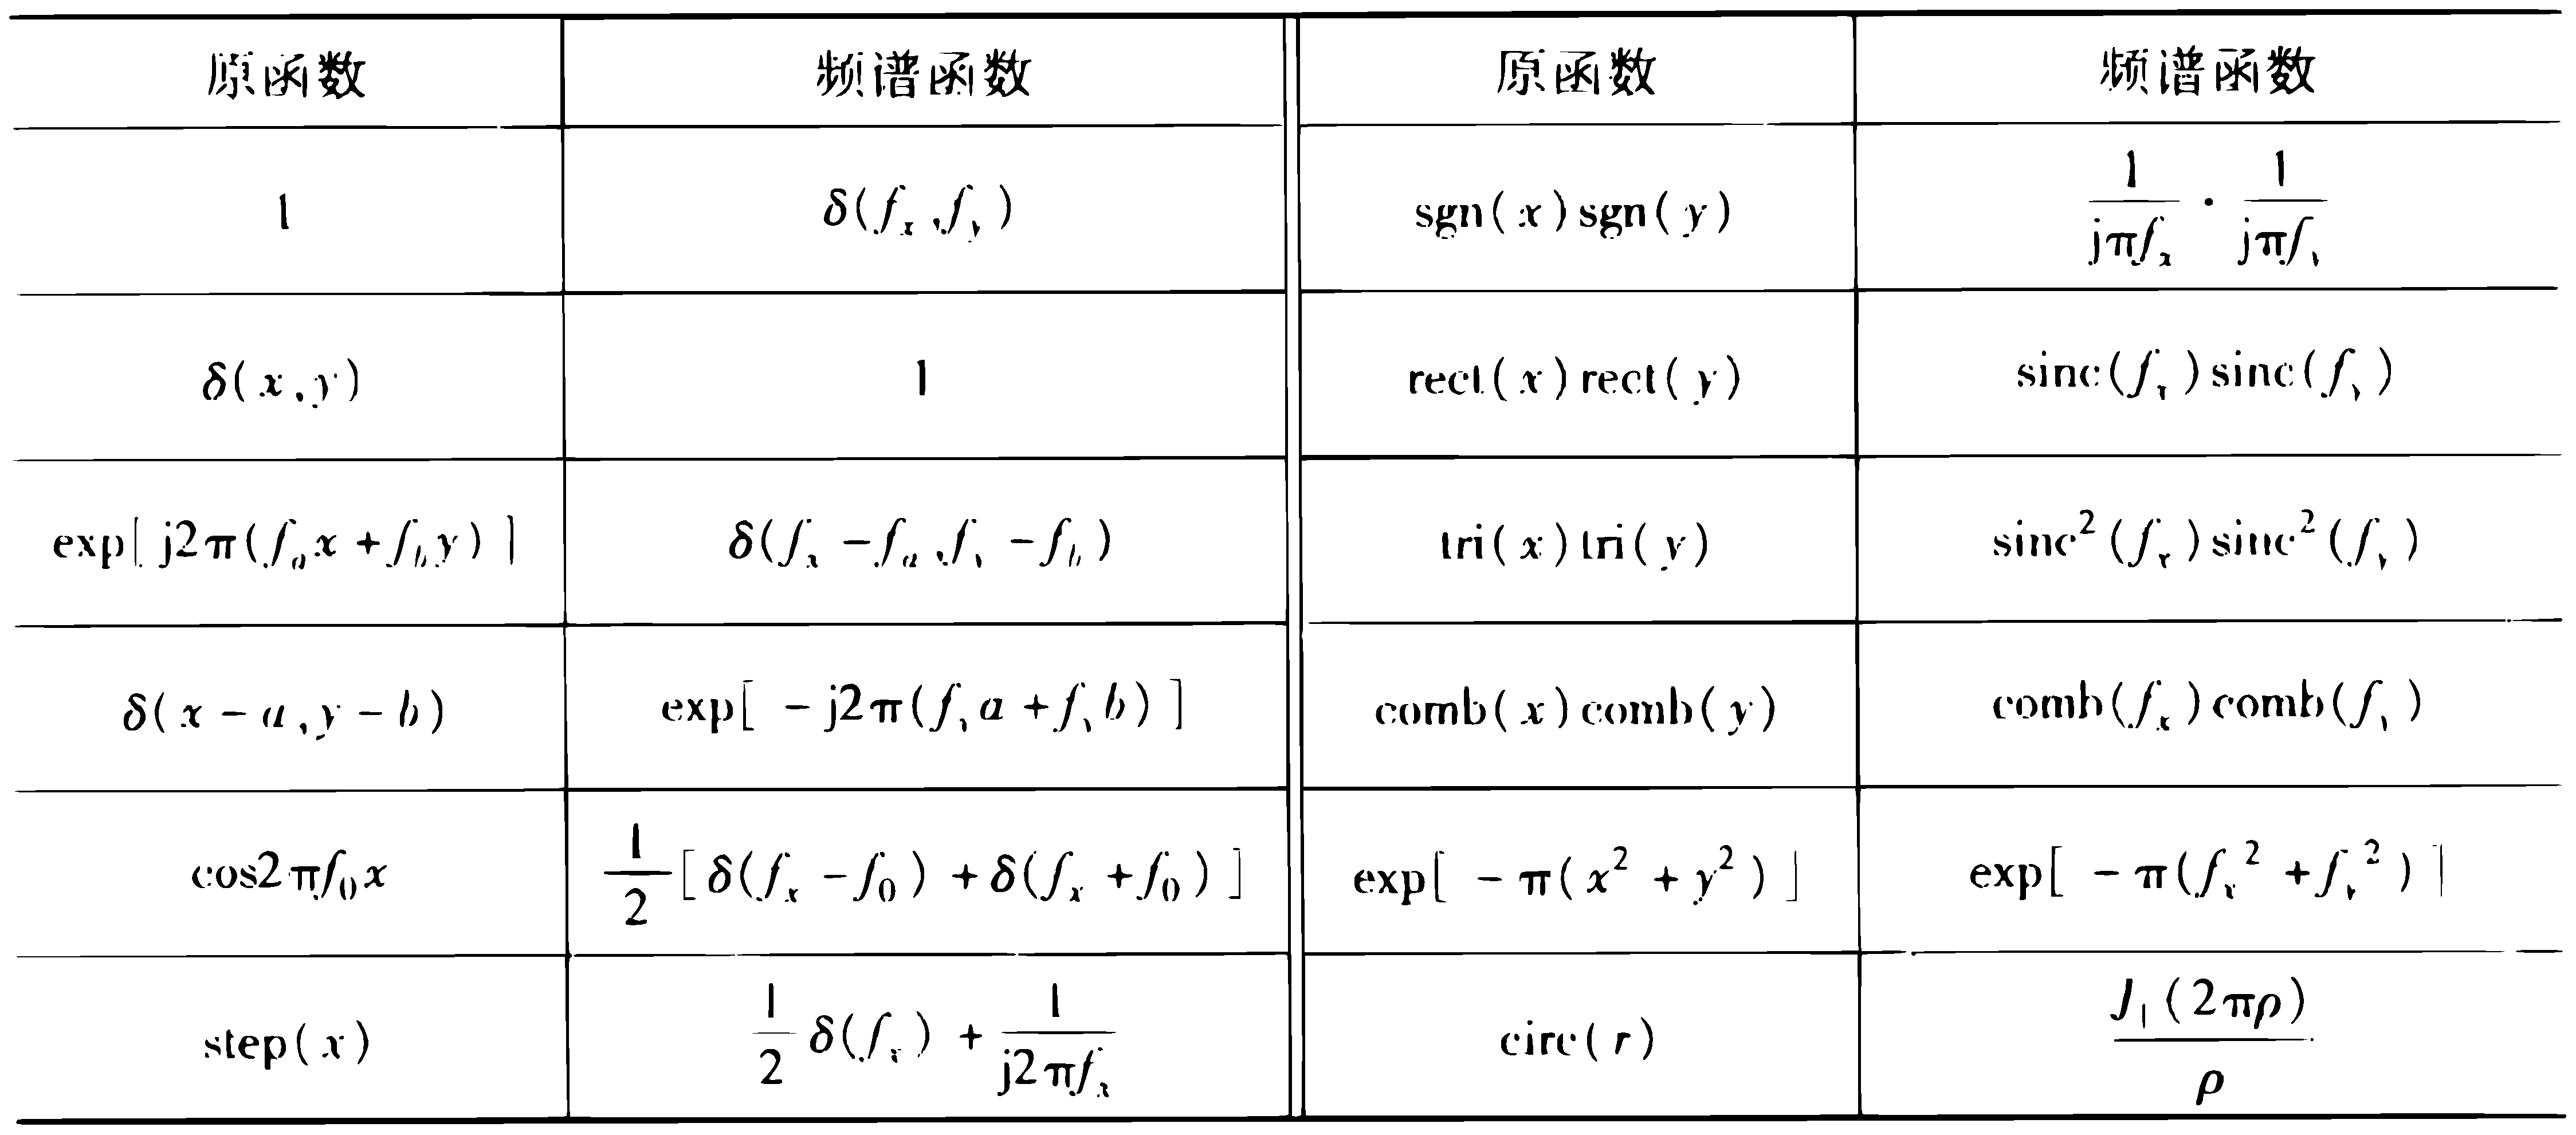
\includegraphics[width=10cm,height=4cm]{graph.eps}
    \caption{傅里叶变换表格}
    \end{figure}    
\end{document}


>>>>>>> e4f7cabd27c4a513469158f610b09335000e40c0
